\section{Coordinate System}
The CMS detector is located on the LHC and is the experiment furtherest from the
CERN Meyrin site; its position on the LHC ring can be seen in figure \ref{fig:LHCRings}
The CMS coordinate system is oriented such that the x-axis points to the center of the LHC
ring. 
%\section{Operation}
%\begin{figure}[t]
%  \centering
%	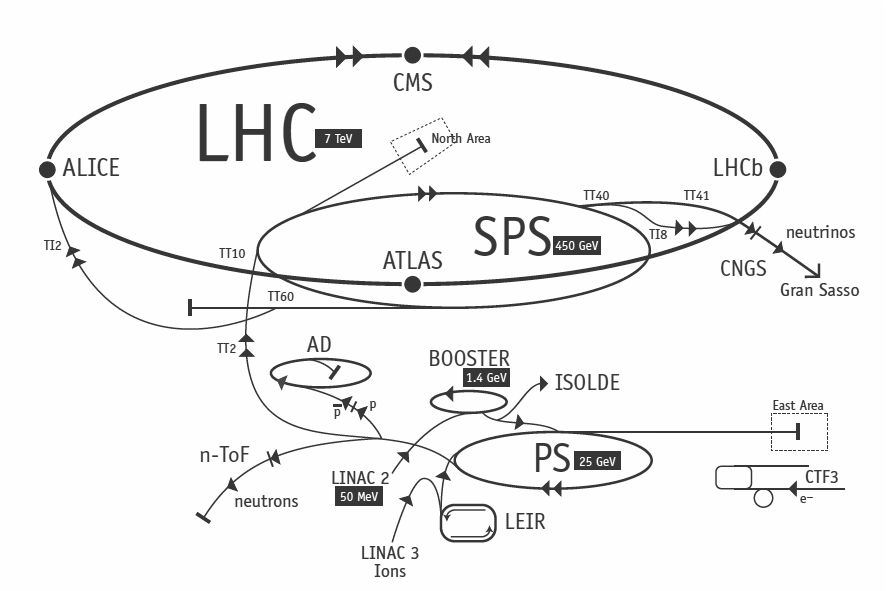
\includegraphics[width=0.75\textwidth]{images/LHCLayout.png}
%  	\caption[e/$\gamma$ LHC Layout]
%   	{LHC and Experiments Layout}
%	\label{fig:LHCRings}
%\end{figure}
The y-axis points vertically upward, perpendicular to the Earth's surface,
the z-axis is in the direction of the beam to the west. The angle $\phi$ is measured
azimuthally starting from the x-axis in the x-y plane, the radial coordinate in this plane
is denoted by r. The polar angle $\theta$ extends in the r-z plane and, importantly,
is used in the definition of pseudorapidity, $\eta$, as, 
\begin{displaymath}
\eta=-\ln{\tan\frac{\theta}{2}}.
\end{displaymath}
The spatial coordinate $\eta$ is preferred over the coordinate $\phi$ for 
defining the angle of a particle relative to the beam axis since
the particle production in minimum bias collisions is constant as a function of $\eta$.
The LHC is a hadron collider, therefore, the energy in the parton-parton interaction
that initiates interesting physics cannot be known. However, it is known that 
the momentum in the direction transverse to the z-axis is ~0. Therefore,
the interesting observables (energy and momentum) are defined as transverse
to the beam by measuring their x and y components and denoted as transverse
momentum, $p_{T}$, and transverse energy, $E_{T}$.%%%add in pt=sqrt(px^2+py^2)^1/2
%Reference: The CMS Collaboration, Detector performance and software, Physics
%Technical Design Report, Volume I (CMS TDR 8.1).
%\end{document}
